% beamer 16:9
\documentclass[aspectratio=169, 9pt, xcolor=table]{beamer}
% suppress the navigation bar
\beamertemplatenavigationsymbolsempty
% add frame number to footline
\setbeamertemplate{footline}[frame number]
% set frame color
% \usecolortheme[named=cyan]{structure}
% set font serif only math
% \usefonttheme[onlymath]{serif}
% set font serif all
\usefonttheme{serif}
\usepackage{subcaption}
% subfile - making directories for slides
\usepackage{subfiles}
% wrapping figures with text
\usepackage{wrapfig}
% table 과 figure 에 번호 붙이기
\setbeamertemplate{caption}[numbered]
% math package
\usepackage{amsmath, amsthm, amssymb}
% code 넣을 때 frame 으로 사용
\usepackage{listings}
% code 넣기
% \usepackage{minted}
% table 에 rule 넣기
\usepackage{booktabs}
% talbe 에 multirow 적용
\usepackage{multirow}
\usepackage{animate}
\usepackage{forarray}
% remove font size error
\usepackage{lmodern}
% hyperlinks
\usepackage{hyperref}
% foreach and other making tools with if and for loop
\usepackage{pgffor}
\usepackage{calc}
\usepackage{ifthen}
% section 만들기
\usepackage{xparse}% http://ctan.org/pkg/xparse
\usepackage{etoolbox}% http://ctan.org/pkg/etoolbox
\usepackage[utf8]{inputenc}
\bibliographystyle{apalike}

\setbeamertemplate{bibliography entry title}{}
\setbeamertemplate{bibliography entry location}{}
\setbeamertemplate{bibliography entry note}{}
\usepackage{kotex}
\usepackage{seqsplit} % for automatic line breaks
\usepackage{graphicx}


% \usepackage[
% backend=biber,
% style=numeric,
% sorting=ynt
% ]{biblatex}
\newcommand{\tred}[1]{\textcolor{red}{#1}}

\DeclareMathOperator*{\argmin}{argmin}
\DeclareMathOperator{\Tr}{Tr}

\AtBeginSection[]
{
\begin{frame}
\vfill
\centering
\usebeamerfont{section title}\insertsection
\vfill
\end{frame}
}

% set theme color
\definecolor{smurf}{rgb}{0.14, 0.39, 0.78}  %%% <- Change it into the color you want
\usecolortheme[named=smurf]{structure}      %%% <- Change it into the color you want

% set title
\title{CPE with Agent Based Modeling}
\author{Kim Sol}
\institute{School of Mathematics and Computing}
\date{\today}
%%%%%%%%%%%%%%%%%%%%%%%%%%%%%%%%%%%%%%%%%%%%%%%%%%%%%%%%%%%%%%%%%%%%%%%%%%%%
\usepackage[style=verbose,backend=biber]{biblatex}
\addbibresource{abmBib.bib}
\begin{document}

\begin{frame}
    \titlepage
\end{frame}
%%%%%%%%%%%%%%%%%%%%%%%%%%START%%%%%%%%%%%%%%%%%%%%%%%%%%%%%%%%%%%%%%%%%%%%%%


\begin{frame}
    \frametitle{Setting}
    The number of iterations is 135
    \begin{center}
    \begin{tabular}{|c||c|c|c|c|c|c|c|c|c|c|}   
        \hline
        \multicolumn{11}{|c|}{Experiment transmission rate (\(10^{-5}\)) } \\
        \hline
        \(\beta\)& 1 & 2 & 3 & 4 & 5 & 6 & 7 & 8 & 9 & 10 \\
        \hline
        patients& 2.26  & 2.54 & 2.14 & 2.30 & 2.50 & 2.57 & 2.58 & 2.44 & 2.71 & 2.65 \\
        \hline
    \end{tabular}
    \end{center}


    \begin{figure}[H]
        \centering
        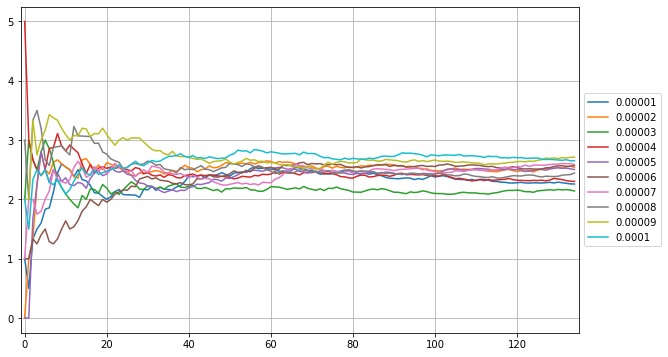
\includegraphics[width=.5\textwidth]{../result/calibration/pic/refinement.png} %must add a space here
        \caption{Cummulative Average number of sick patients}
    \end{figure}
    
\end{frame}

\begin{frame}
    \frametitle{Result}
    The values between \(10^{-5}\) and \(10^{-4}\) were subdivided and tested. 
    \begin{figure}[H]
        \centering
        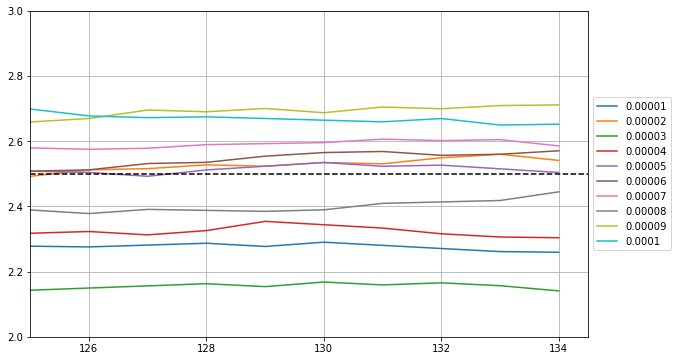
\includegraphics[width=.5\textwidth]{../result/calibration/pic/refinement_zoom.png} %must add a space here
        \caption{Cummulative Average number of sick patients}
    \end{figure}
    As a result, all values did not increase sequentially. The value at 3 was the lowest, the value at 2 was similar to the target value, and the value at 8 was surprisingly small. Excluding these, 1 and 4 showed relatively low average values, 5,6,7 showed intermediate values, and 9 and 10 showed high values.
\end{frame}



% \begin{frame}
%     \frametitle{Controls}
    
%     \begin{itemize}
%         \item Environment cleansing
%         \item HCW route (eg. visit isolated beds only? or both?)
%         \item Handwashing probability (from literature, fixed at .9)
%         \item Isolation of infected patients
%     \end{itemize}
% \end{frame}

\begin{frame}
    \frametitle{Questions}
    
    \begin{itemize}
        \item I wonder if it is appropriate to use 0.00005 as the $\textit{transmission probability}$.
        
    \end{itemize}
\end{frame}
% \begin{frame}
%     \frametitle{Attempt to view the long run equilibrium}
%     \begin{figure}[H]
%         \centering
%         \includegraphics[width=.5\textwidth]{../../../ref/figures/abm_longrun.png} %must add a space here
%         \caption{Sample run}
%     \end{figure}
%     \begin{itemize}
%         \item Notice that in the long run, almost every bed that the HCWs visit ends up being sick
        
%     \end{itemize}
% \end{frame}

% \begin{frame}
%     \frametitle{Some ideas for control}
%     \begin{itemize}
%         \item Set routes and find the optimal partition
%         \item Make best use of isolated beds
%         \item Environment cleansing
%         \item Max handwashing; but this would imply, in theory, no infection within the ICU
%         \item \textit{Need a baseline to compare the strategies}
        
%     \end{itemize}
% \end{frame}


\end{document}



